\section{Test Setup}
\label{sec:testsetup}
\subsection{Hardware}
\label{sec:hardware}
This section introduces the hardware setup created in order to validate our chip design and compare the received samples with the results obtained from simulations. For an as like to like comparison with the simulations as possible, the hardware tries to replicate the virtual test bench setup. As in the virtual setup, the physical setup contains electronically controllable loads to compare the dynamic regulation characteristics with the simulated results. The response to load steps also gives insight into the closed loop regulation characteristics like bandwidth and phase margin of the internal regulation loop. An additional goal is to verify our SPI slave implementation with a commercial SPI master device like an Arduino or USB to SPI converter. Of additional interest is the accuracy of internal signals such as the internal oscillator and the the bandgap voltage reference.\\
The hardware should allow for the following measurements:
\begin{itemize}
    \item Line Regulation
    \item Load Regulation
    \item Output Voltage Regulation Accuracy 
    \item Efficiency
    \item Startup Behavior
    \item Short Circuit Behavior
    \item SPI Functionality
    \item Internal Oscillator Frequency Accuracy
    \item Bandgap Voltage Reference Accuracy
\end{itemize}

Continuing the test bench analogy, the test setup is split into two components, a test bench like \ac{PCB} we call the Adapter \ac{PCB} and multiple smaller \ac{PCB}s. These smaller \ac{PCB}s only contain the \ac{DUT} and a minimal amount of supporting components for its orderly operation. As these \ac{PCB}s get plugged in on top of the Adapter \ac{PCB}, we refer to them as Hats.

\clearpage

\subsubsection{Adapter PCB}
The main Adapter \ac{PCB} contains the functionality of the test bench and has a common plug-in location for the Hats. The Adapter is designed in such a way, that the \ac{DUT} can be placed in the thermal chamber of the thermal airstream system TP04300A in order to test the \ac{DUT}s functionality under various thermal conditions. Four electronically controllable load resistors are contained on the \ac{PCB} for load step measurements and current sense amplifiers are used to measure the current flowing into and out of the switching converter. In order to verify the SPI communication with the \ac{DUT}, there are headers and voltage translators for communication with either an Arduino Nano Every or an FTDI FT232 based USB to SPI adapter.

\begin{figure}[h]
    \centering
    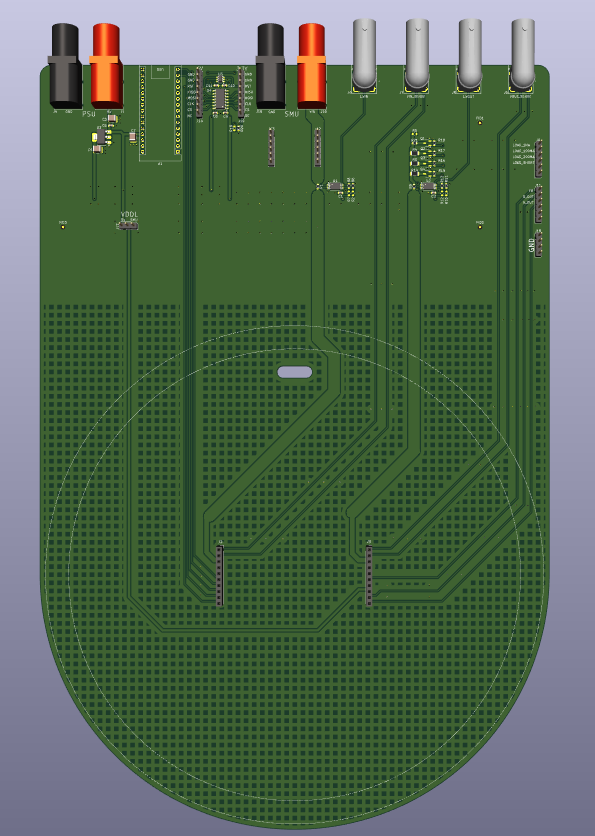
\includegraphics[width=0.6\textwidth]{../ASIC-DESIGN-2/images/02_test_setup/Adapter _PCB.png}
    \caption{3D render of the Adapter PCB, the design files can be found in the following git repository \cite{PCB_schematic}}
    \label{fig:Adapter_PCB}
\end{figure}

\clearpage

\subsubsection{Hat PCB}
In total three different Hat \ac{PCB}s were created in order to test various \ac{DUT}s. One \ac{PCB} contains a commercially available \ac{IC} and the two other \ac{PCB}s are inteded for our manufactured chip. On the first \ac{PCB} our chip is placed into an \ac{IC} socket and in the second one the QFN package soldered directly to the board. The socketed version allows for the quick characterization of multiple samples and measurement of the variance of characteristics over the batch. The socket however introduces higher lead resistances and inductances as well as thermally isolates the chip from the \ac{PCB}. The thermal isolation could lead to increased temperatures in high load conditions and in a worst case scenario could lead to damage of the chip. In practice however, no a measurable difference in characteristics was observable based on if the chip was socketed or not.\\


\begin{figure}[h]
    \centering
    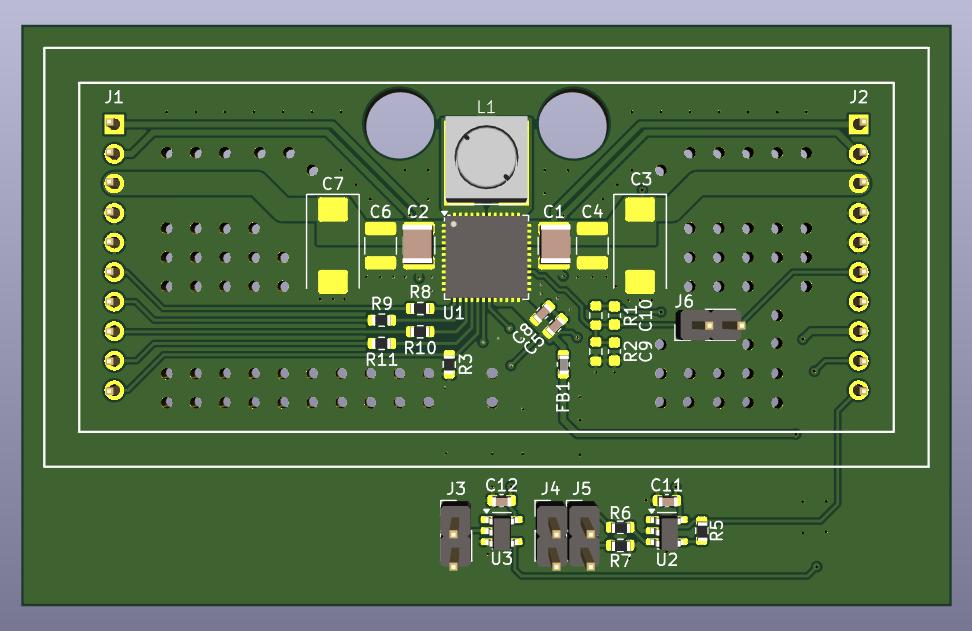
\includegraphics[width=0.75\textwidth]{../ASIC-DESIGN-2/images/02_test_setup/ASIC_Hat_PCB.png}
    \caption{3D render of the Hat PCB with the QFN package soldered to the PCB, the design files can be found in the following git repository \cite{PCB_schematic}}
    \label{fig:ASIC_Hat}
\end{figure}


The reasoning to create a Hat with a commercially available chip was two fold. First it allows validation of the test setup with a real hardware before receiving samples and secondly it creates a baseline to compare our design against. For the commercially available \ac{IC} we used the TPS63900 from Texas Instruments. While this \ac{IC} is significantly smaller in physical size, it has a similar input and voltage range as well as current drive capabilities. Similarly it is also a highly integrated buck-boost converter with integrated switches in the standard cascaded-buck-boost converter topology. Nonetheless the TPS63900 has a significantly higher efficiency, greater than \qty{90}{\percent}\cite{tps63900}, as it is designed for ultra low-power applications and implements multiple advanced power saving features like dynamic switching frequency adjustment based on load conditions\cite{tps63900}. The chip additionally employs a novel drive scheme of the power stage leading to trapezoidal inductor current, as opposed to the traditional triangular waveform, which again leads to higher efficiency and to only a single operating mode over the entire input and output voltage range\cite{tps63900}. 